\chapter{Introduction}\label{chapter:intro}


\chapterintro*
This chapter provides the reader with a background in the industrial revolutions of the past up until the present.  It provides a context by which the reader may understand more fully the impacts of the contributions presented within this thesis.  The chapter begins with a brief historical perspective followed by an introduction of smart manufacturing.  This introduction is necessary of the reader to understand the challenges of employing wireless technology in a factory and why the contributions of the thesis matter are important.

\section{Industrial Revolutions}
Major advances in manufacturing of goods for the betterment of humanity have occurred many times in the last two hundred and fifty years in the history of humanity.  These advancements occurred of science and technology occurred as revolutionary events at different times.  The first revolution occurred at the edge of the eightieth century primarily in England but also in France, Germany, and the United States with the applicant of automatic mechanization of large machines using coal powered steam engines.  These machines were mainly used for the processing of cotton, wool, and silks in the production of textiles for export throughout the world.  Advancements during this period included uses of coal to produce steam power, the production of iron, steel, and other rudimentary alloys, and, very importantly, the engineering advancements of tool making.  The advancements of the first industrial revolution paved the way for the centralization and mass production of goods.
%CITATION SOURCES *** {https://en.wikipedia.org/wiki/Technological_revolution#Potential_future_technological_revolutions}

The next century was marked by the development of scientific and engineering advancements in chemistry, physics, and engineering. Experimentation with electricity and the production thereof led to the eventual explosion of industrial machinery, tooling, electrification, chemical manufacture, petroleum refinement, rail and marine transportation, the automobile, agriculture, and telecommunications by wire over long distances.  This period of discovery culminated with rapid expansion of industrialization through the world, especially in North America and Japan up until the beginning of World War I.
%CITATION SOURCES *** https://en.wikipedia.org/wiki/Second_Industrial_Revolution#Machine_tools

\begin{figure}[!tbp]
	\begin{center}
		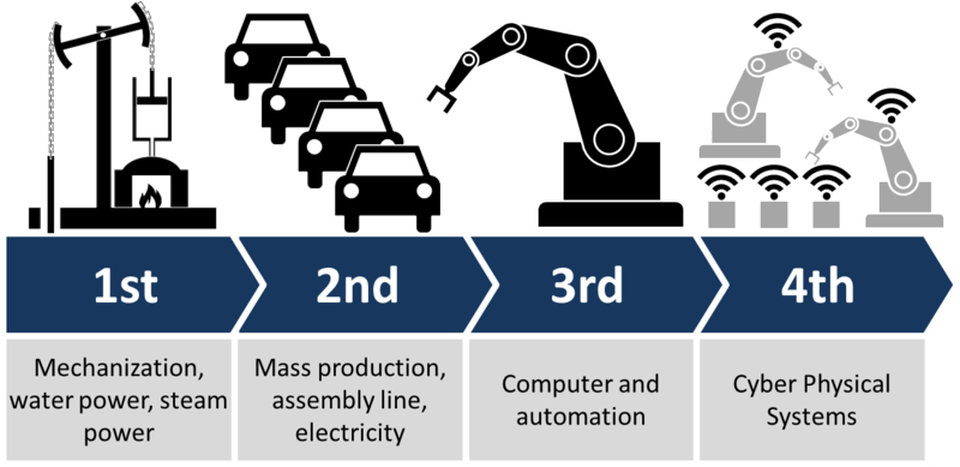
\includegraphics[width=0.75\textwidth]{chapter-intro/images/forbes_2016_03_Industry_4.0}
		\label{fig:intro:forbes-i40-evolution}
		\caption{Industry 4.0: Wireless is a key enabler in the 4th industrial revolution.}
	\end{center}
\end{figure}

The third industrial revolution began in the tears immediately following the second world war with the rapid advancement of pure and applied sciences.  These advancements were driven primarily by the cold war and the space race between the United States and the USSR.  This period of advancement was marked by many discoveries and scientific applications such as the development of telecommunications theories (Claude Shannon), advancement of radio and wired communications, the discovery of the transistor, and the rapid expansion of computers and information technology in business and defense.  Also during these years, arrived the application of computing within manufacturing and process control settings. Computers slowly began to replace the basic relay circuit in control systems.  By utilizing the programmable logic controller (PLC), manufacturers gained the ability to develop control their processes more easily and develop control strategies that were once more difficult to implement in the past with dedicated, specialized equipment.  PLCs offered both the ability to more easily adapt processes to information gathered directly from the factory operation as well as slowly collect and store information electronically.  However, electronic storage of this information was still both difficult and expensive as telecommunications technology was yet relatively slow and storage expensive.  Over the years following through the 1980's until today, computers have followed closely Moore's "Law" which states according to the the perception of Intel Corporation founder, Gordon E. Moore, that the number of transistors on a microchip doubles every two years.  This paradigm of exponential growth in digital computing technology in terms of computing speed, storage, and efficiency has created a world in which computers and computing devices have become ubiquitous, surrounding practically every aspect of human endeavors and leading to the latest installment of industrial advancement, the 4\textsuperscript{th} Industrial Revolution, also known as the \textit{Information Revolution} which is currently ongoing. 

The Information Revolution is defined by a culture that is highly interconnected and data depended.  Clearly, the modern world is dominated by the Internet, high-performance computers, and personal mobile communications devices such as cell phones developed over the last several decades. Within the hands of each individual one may find a smartphone capable of performing computing and communications tasks not even imaginable fifty years ago.  Indeed, within each of these devices resides a powerful microprocessor capable of clocking speeds in the gigahertz, offline storage spanning gigabytes, at-least one high-resolution camera, and communication components enabling high-speed connectivity capable.  These personal devices are smart and easily re-programmable by downloading of new applications, i.e., \textit{apps} enabling users to produce and consume information rapidly.  Users enjoy the ability to speak at any moment, send brief messages using apps such as WhatsApp\texttrademark, download videos, play games, store documents, music, photographs, and videos within "the cloud."  Within office and business enterprises, a personal computer is within reach of every employee and is the tool used for information production.  The data produced is stored within the cloud and usually produced and maintained locally, although the services of data production are quickly shifting to the cloud as well depending on the needs the end user.

These capabilities have also been permeating industrial environments although at a slower rate given the inherent conservatism of industrial establishments.  Industrial environments include aerospace and automotive manufacturing, electrical power production, food processing, petroleum and chemical production.  That is not to say that industrial establishments are not open to technological change, but that established production system can be difficult or risky to modify once they are operational.  While industrial operations have distinctly different requirements than office businesses; analogues may be made between the computing constructs found within the personal/business computing domains and those constructs founds within the industrial computing domains.  For example, within a factory production enterprise, the Internet itself exists as an outside entity providing global connectivity, hosting, storage, computing resource, and analysis tools.  These services are often replicated within the business enterprise of the factory operation and extended into the factory environment to some degree from the factory management system to the factory floor.  

In addition, with the explosiveness of ubiquitous, low-cost computing devices, the modern factory operation is changing to include more intelligence and adaptability at the factory edge.  This includes discrete devices such as sensors and actuators, collaborative robots, autonomous gantry systems, intelligent vehicular systems, tracking and inventory systems, and the like.  These systems coupled with the plethora of computing resources have the potential to create an enormous amount of information as well as the opportunities for greater control over the factory enterprise.  It is just a matter of tapping the information within the factory and bringing that information to a useful purpose.  Where the third industrial revolution brought computing and automation to the factory, the fourth industrial revolution will improve upon the automation found within the factory by adding intelligence, autonomy, and machine learning powered by data. This datacentricty defines Industry 4.0.  

\section{Industry 4.0 and Smart Manufacturing}
Industry 4.0 also known as "smart manufacturing" was \textit{officially} launch by President Barack Obama of the United States and Chancellor Angela Merkel of Germany at the Hannover Messe industry show on April 24, 2016{\cite{HannoverMesse2016:Report, HannoverMesse2016:MachineDesign}.  Smart manufacturing is a term used to described the ongoing efforts within academia, government, and private industry to improve upon existing and future factory operations by incorporating the latest advances and design principals in computing, storage, and communication such as interoperability, virtualization, decentralization, distributed control, real-time processing and communication, service oriented architecture, easy use and maintenance, cost savings, and modularity of design.  With I4.0, the industrial internet of things (IIoT) and industrial cyber-physical systems are expected to make large sweeping changes in efficiency, reliability, and capability of the future factory~\cite{Raptis2019}.	

\begin{figure}[!tbp]
	\begin{center}
		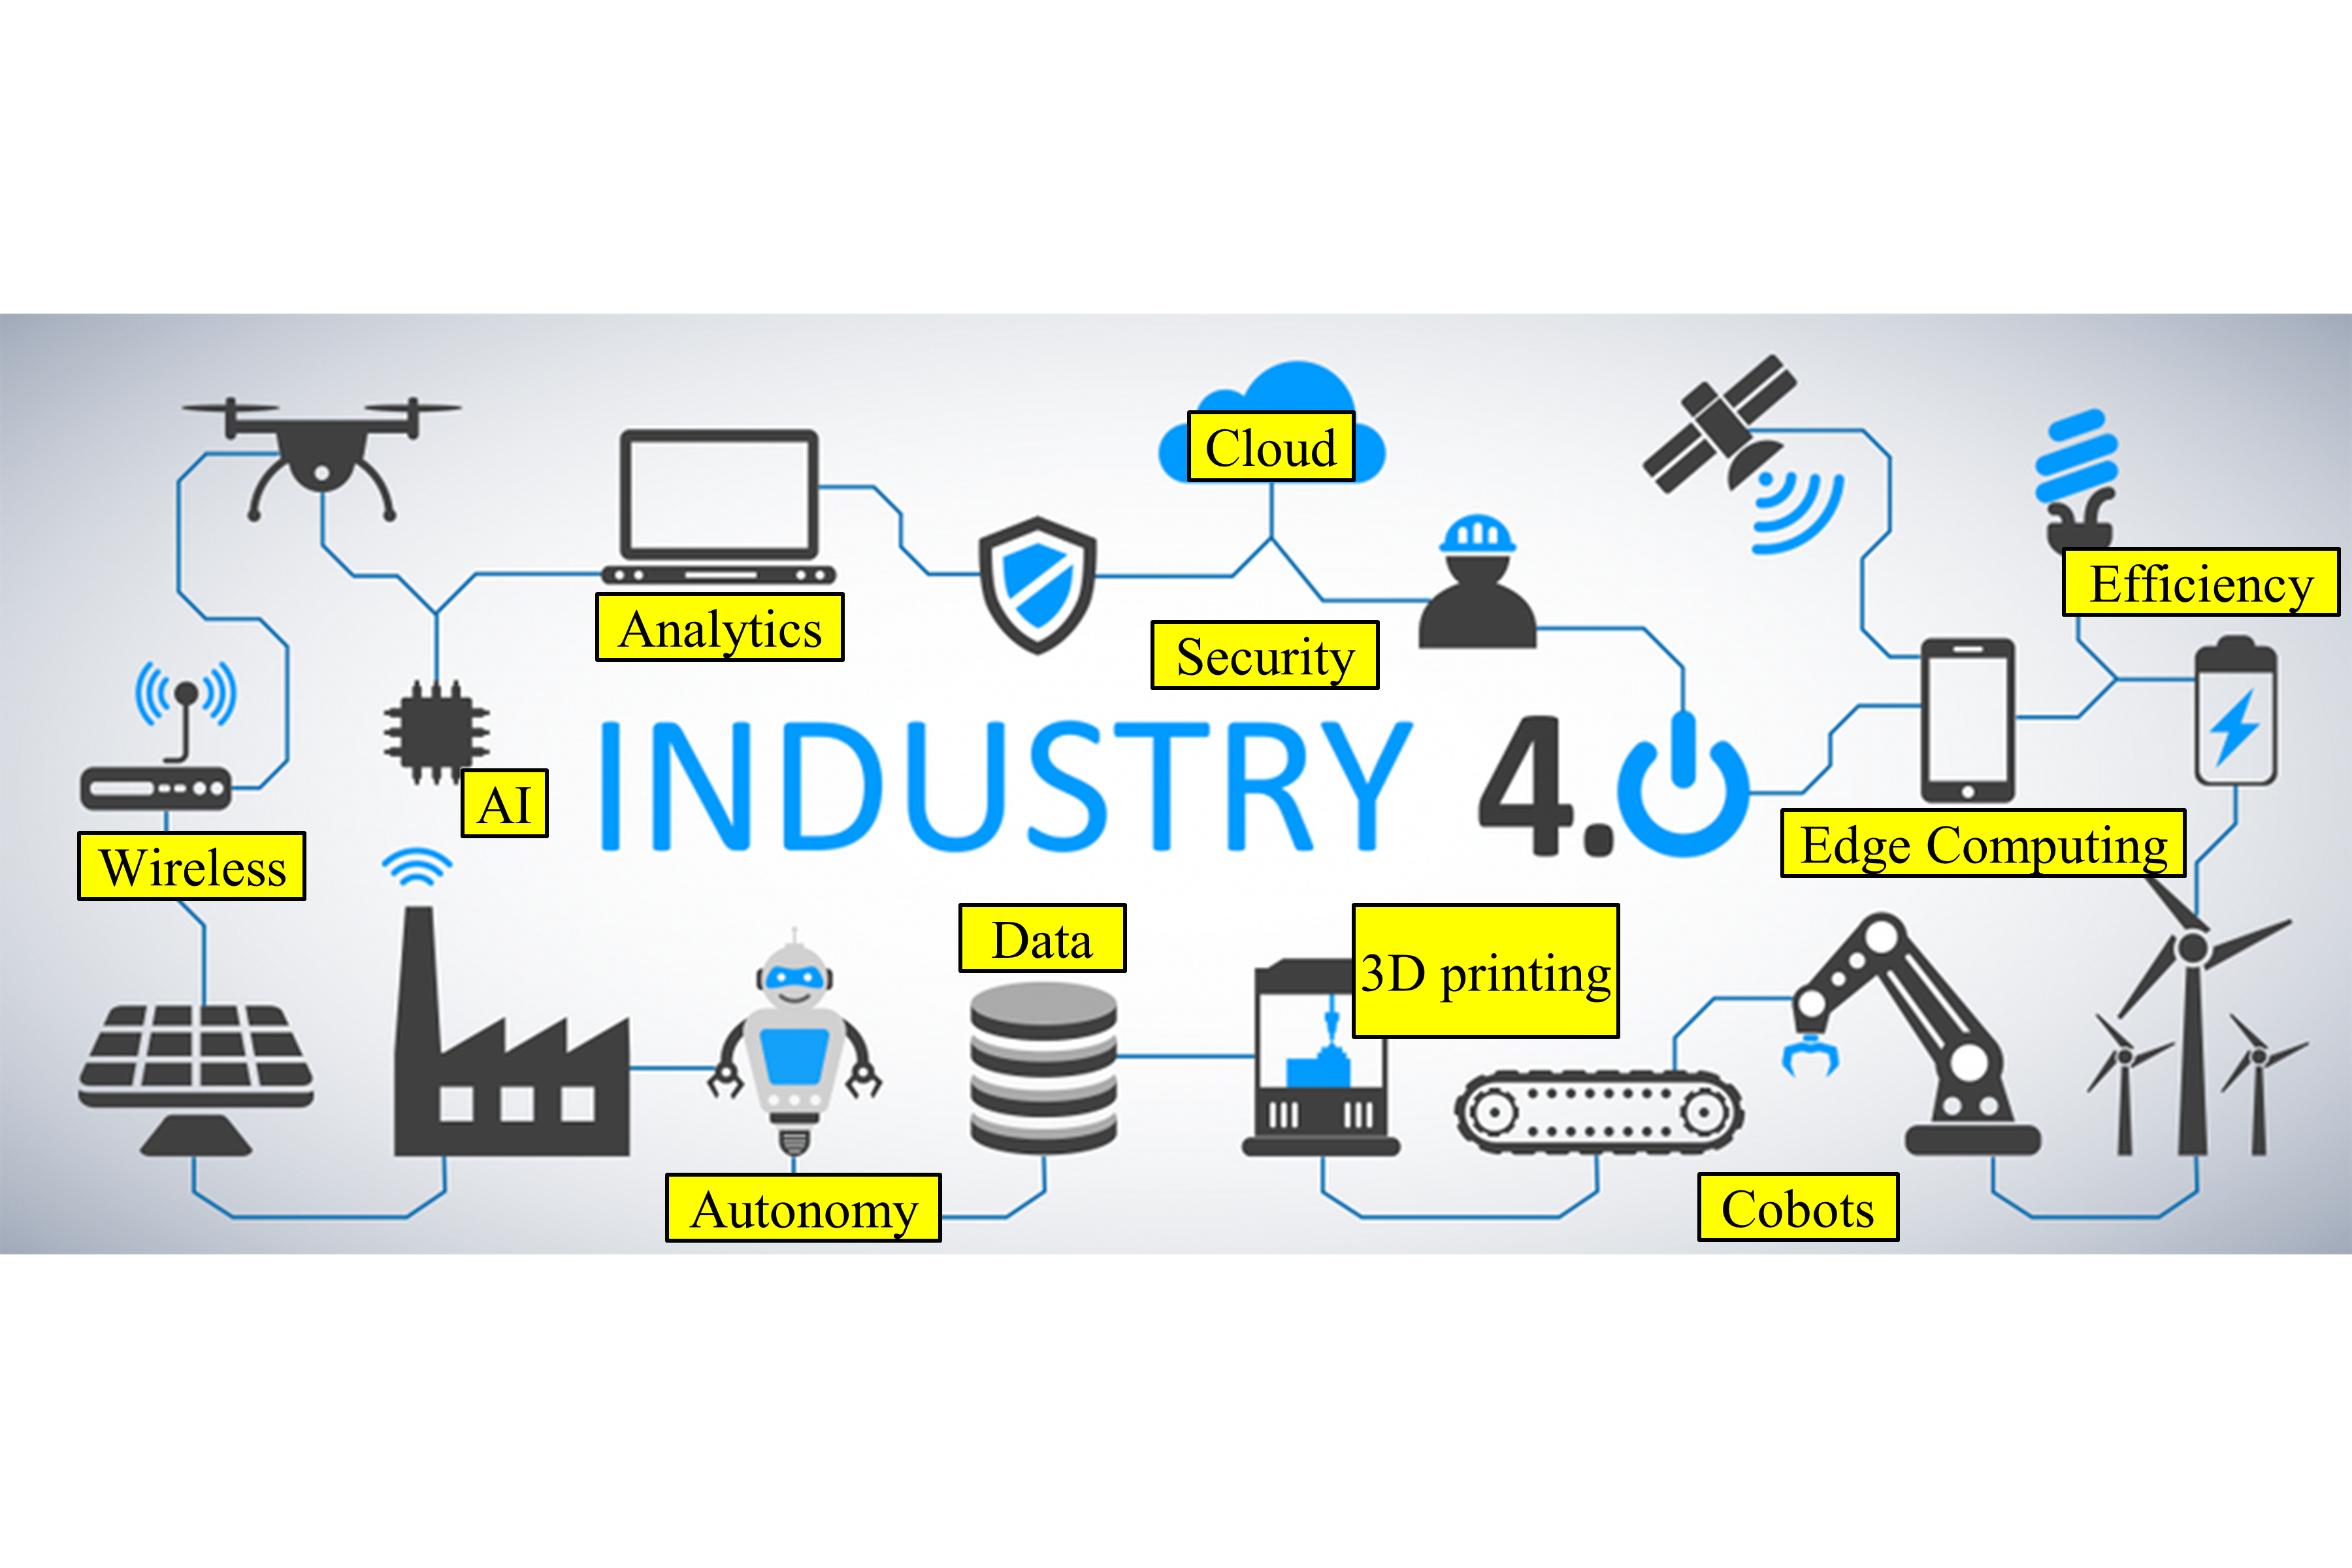
\includegraphics[width=\textwidth]{chapter-intro/images/intro/forbes-i40-candell.png}
		\label{fig:intro:forbes-i40}
		\caption{Industry 4.0: Incorporating the benefits of machine learning, massive data, mobility, and autonomy within the modern factory.}
	\end{center}
\end{figure}
\begin{verbatim}https://www.forbes.com/sites/bernardmarr/2018/09/02/what-is-industry-4-0-heres-a-super-easy-explanation-for-anyone/#6dee527a9788\end{verbatim}

Propelled by economic pressure toward greater efficiency, factory agility, and product customization, future factories will have the technological ability to adapt to customer demands quickly, modify manufacturing processes automatically based on quality feedback, and fabricate products with a reduced environmental impact.  Technological advances required for smart manufacturing to be truly successful include a collaborative and mobile robotics, distributed machine autonomy based on artificial intelligence, and a high degree of interconnectivity of among the automation resources.  Robots will work together and with people to accomplish complex tasks.  Robots will have the ability to roam between work-cells within a factory, learn its role quickly, become aware of edge devices, and communicate with other actors within the work-cell to accomplish its goals.  Current manufacturing architectures use wired connectivity through field bus and industrialized Ethernet for sensing and real-time control.  

\section{The Importance of Wireless in Smart Manufacturing}
The concept of Industry 4.0 is centered around the smart factory in which autonomous actors permeate the factory.  Wireless technology is an essential requirement for all interconnected things that are wireless. Cyberphysical systems (CPS), i.e., systems in which the networking, computation, and the physical world are tightly integrated will dominate the factory.  Whereas as the factory of the past was predicated on centralize design making based on limited data and knowledge of the past, present, ad future state of the business enterprise, decision making within the smart factory will be highly decentralized.  Information will likely be stored in the cloud; however, the actors making decisions will be located in throughout the factory itself at the edge.  Wireless technology will be used fore two main categories within the smart manufacturing enterprise and are described as follows:

\begin{description}
	
	\item[Cable Elimination] Substitution of a wireless technology where once a wire existed in an existing industrial system.  This often occurs when the cost of installing a cable is either infeasible or prohibitively expensive but the cost of not replacing the wire would cost more.  This type of system could be envisioned where once a cabinet existed as a nexus point for fieldbus input-output (I/O) end-points.  If a legacy product fails thus rendering the nexus in-operational, wireless could be used to replace the connections between a computing device and the various I/O endpoints.  This scenario is often cited in industry as a high-likelihood scenario for both sensing applications and sensing with control applications where the I/O end-points are stationary.  Wireless will be used to circumvent future failure or will be used as a rapid replacement measure for a failed system.
	
	\item[Mobility Enabling] Support of one or more untethered actors such as a robotic arm or heavy lift machine to assist in the movement of materials or the tending of other processes.  In these applications, the untethered actors require, at a minimum, instructions to perform their tasks.  More than likely, the mobile actor will need to remain aware of itself and its surroundings, communicate to a supervisor or other mobile actors.  Interconnection with the factory safety systems will likely be a necessity.
	
\end{description}


\section{Challenges in Industrial Wireless Networks}
Since the development of wireless sensor networks (WSN) beginning in the early 2000's much excitement has been generated by its promises~\cite{OnWorld2014}.   Development of IEEE 802.15.4~\cite{wiki:ieee802.15.4} brought about such standards as WirelessHART~\cite{Song2008}, ISA100.11a~\cite{ISA100.11a}, and Zigbee as low-power mesh networking options for industry.  Other similar wireless networking technologies include LoRAWAN, Sigfox, 6TiSCH, and WiFi to name a few.  These WSNs technologies were all designed primarily with the main goal of collecting information or transmitting large amounts of data rapidly in the special case of WiFi.  They were not really intended to command or control devices, although they have been at times adapted to do so.  For example, WirelessHART and ISA100.11a have the primitives (i.e., the "hooks" to do so) and some valve control and other applications have been realized using these protocols.  These types of WSN technologies were designed to support sensing with some supervisory or human-in-the-loop control with command decisions rarely occurring and without demanding reliability or latency requirements placed on the communication system.  Indeed, the wireless sensor networks typically operate with 75\% link-to-link packer success rates at the physical layer.  With the advent of 5G communications which in this context includes both cellular and wireless local area networks (WLAN) such as Wi-Fi (e.g., IEEE 802.11ax), much work has been done to characterize the wireless requirements landscape for industry as summarized in~\cite{Montgomery2019}.  The requirements landscape for industrial wireless can be organized into to main categories: 1) sensing and data gathering, and 2) control.  For the first category, many technologies already exist to support these applications, and rarely is reliability or latency a major concern for these applications.  The second category, control has garnered interest within the academic and industrial communities because of the promises of eliminating cables and enabling mobility, and hence, autonomy.  

However, adoption of wireless for control applications has been rare to date~\cite{Martinez2019}.  The primary reasons for its evident failure is most likely reluctance on the part of control designers to use a mode of communication that on the surface appears brittle and unreliable regardless of the truthfulness behind these assumptions.  Wireless technology in general has the following perceived shortcomings that need to be addressed by the research and development community before its widespread adoption comes to fruition.  These shortcomings include the following:

\begin{description}	
	
	\item[ChoiceS, Obsolesence, Interoperability] Many wireless alternatives exist, and the market is ever changing.  The number of choices can be confusing for factory operators trying to implement a solution that will last 10 years or more.  In comparison, wired networks are typically built on the same Ethernet or fieldbus backbones that have existed for decades. When factory control engineers select networking equiment for a factory installation, they intend for those devices to last for at least 10 years or more.  With a plethora of selections in the wireless market, the marketing hype surrounding those devices, and the rapidity by which technology changes, the reluctance to adopt wireless becomes clear.  
	
	\item[Reliabilty (Link Performance)] Information flow between actors within a factory operation.  Since wireless communication is by definition communication without wires across a shared physical medium, it is perceived (correctly) that wireless is not reliable.  This perception of a difference in reliability fuels the reluctance of wireless adoption within factories although the strong desire exists to do so.
	
	\item[Security] Factory operators want their networks to have the same level of security as their wired networks.  The very nature of wireless is open in terms of access ot the physical communication media.  Essentially, this leaves wireless open for eavesdropping attacks assuming that the underlying encryption can be hacked.  If strong encryption is used, the wireless network can still be compromised by jamming or interference.  Security of the wireless network includes immunity from interference, fitness of data, and privacy.  Indeed, the concept of security can be extended to include all aspects of reliability, data integrity, privacy, safety, and stability of the factory operation touched by the wireless network.	
	
\end{description}

The use of wires precludes mobility and makes deployment of edge devices more expensive as each devices requires power, wires, and conduit for communication. By adopting wireless for both sensing and control of machines within the work-cell, a lower-cost, untethered operation becomes achievable. Once wireless is adopted as the primary mode of communication, questions arise as to the required latency, reliability, scale, and security of the wireless network especially when the network is used for the control of machines and the assurance of safety. 

In a factory operation where wireless is used as a primary mode of communication, performance of the wireless network becomes paramount and the ability to assess that performance becomes equally important.  Performance of the wireless network depends on many factors that are impossible to define here within this thesis; however, an introduction on industrial wireless deployments which includes an excellent primer on radio communication can be found in~\cite{Candell2018.IWSGuide} for which the author of this thesis was the primary contributor.  Nevertheless, the main categories of factors that impact an industrial wireless network are provided as follows.


\paragraph{Wireless Protocols Used} Each wireless protocol has been designed with its own target application and ambient environment for performance.  Each protocol is designed with a method for accessing the radio media, organizing data for transmission, methods for receiving transmissions, and recovering from interruptions.   For example, IEEE 802.11 also known as Wi-Fi was designed primarily for home and office use for the transfer of large amounts of data rapidly.  Wi-Fi typically uses 20 to 40 MHz of bandwidth and employs high order modulation and coding schemes.  Wi-Fi works well to transfer files and stream video, and serves well where traditional Ethernet is used; however, Wi-Fi operates within public radio bands and is prone to interference, contention, and non-determinism of response times.  In contrast, other protocols such as WirelessHART and ISA100.11a are designed specifically for industrial wireless sensor networks.  These protocols use low-order modulation schemes with frequency hopping and are by design more resilient to interference.  They are also offer substationally better determinism but are limited in data throughput.

\paragraph{Propagation Loss} Wireless communication as compared to wired modes of communication is considered "lossy".  The probability of error for any wireless communication is governed by the amount of power detected by a receiving radio and the competing noise and interference observed by the receiver.  It is essentially and matter of maintaining an acceptable signal-to-noise ratio (SNR). The amount of loss between a transmitter and receiver is governed by the general equation $L=10\log_{10}\left(\left(\frac{4\pi d f}{c}\right)^2\right)$ where $d$ is the distance between transmitter and receiver and $f$ is the frequency transmission.  Thus, the SNR drops with distance for a given frequency.  Whereas cables typically experience very little loss, wireless modes of communication experience loss very rapidly depending on the frequency of transmission as shown in Fig.~\ref{intro:pathloss-example} as negative path gain.  The figure shows the typical loss curve for a particular factory at 2245 MHz near the common 2400-2500 MHz Industrial, Scientific, and Medical (ISM) band used by WiFi, Zigbee, and WirelessHART, ana ISA100.11a.

\begin{figure}
	\centering
	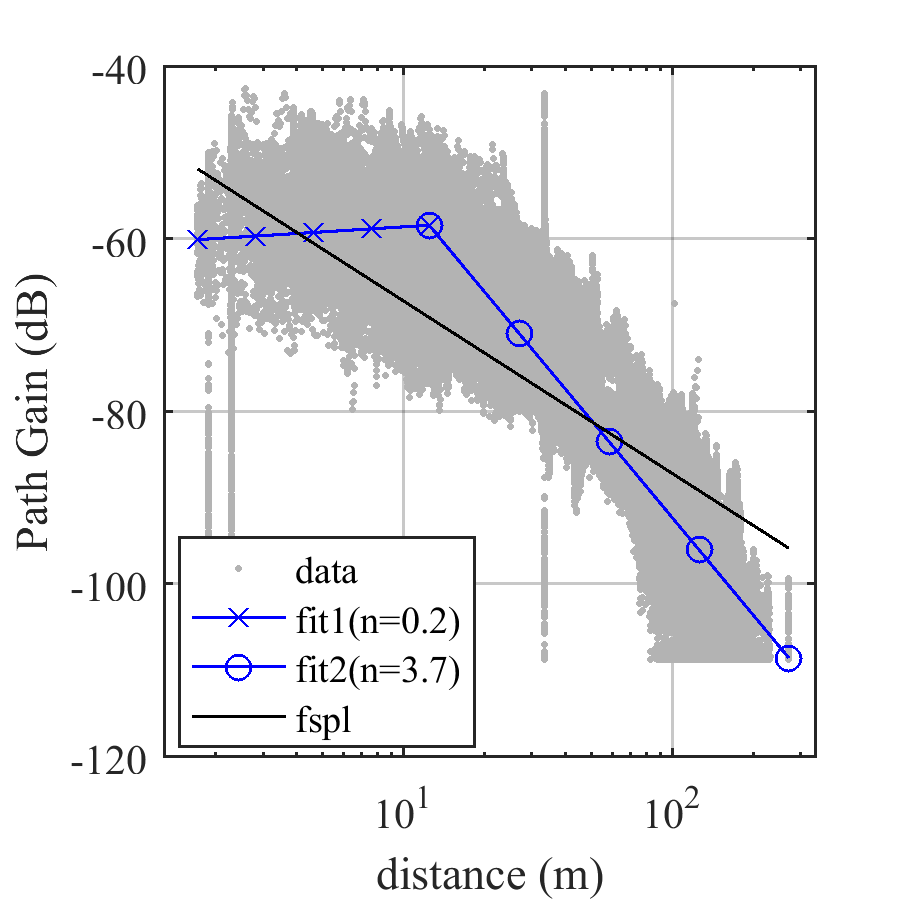
\includegraphics[width=0.6\textwidth]{chapter-intro/images/gain2245}
	\caption{Example of radio propagation path loss for 2245 MHz transmissions within a factory environment.  Reproduced from NIST Technical Note 1951~\cite{Candell2017.NIST1951}}
	\label{intro:pathloss-example}
\end{figure}
 
\paragraph{Multi-path} Objects within the surrounding environment determine the behavior of the waves as they propagate through the environment.  Shown in Fig.~\ref{intro:fig:multipath}is a simplified model of a radio channel. When RF energy is transmitted, it will travel in the direction determined by the antenna gain pattern.  Objects in the environment may obstruct, attenuate, or reflect RF energy.  Reflections contribute to a phenomenon known as multi-path.   Edges of objects may also result in diffraction even if a line-of-sight (LOS) path exists.  At the receiver end, direct path and reflected energy is detected and decoded into useful information if the signal energy was high enough to overcome naturally and artificially occurring noise and interference.  Multi-path reflections may result in significant information loss even if signal power is high.  Multi-path is severe within factories due to the large highly-metallic structures that exists in those environments\cite{Candell2017.NIST1951,Rappaport1991,Remley2008}; therefore, industrial wireless system must anticipate and accommodate these effects.

\begin{figure}
	\centering
	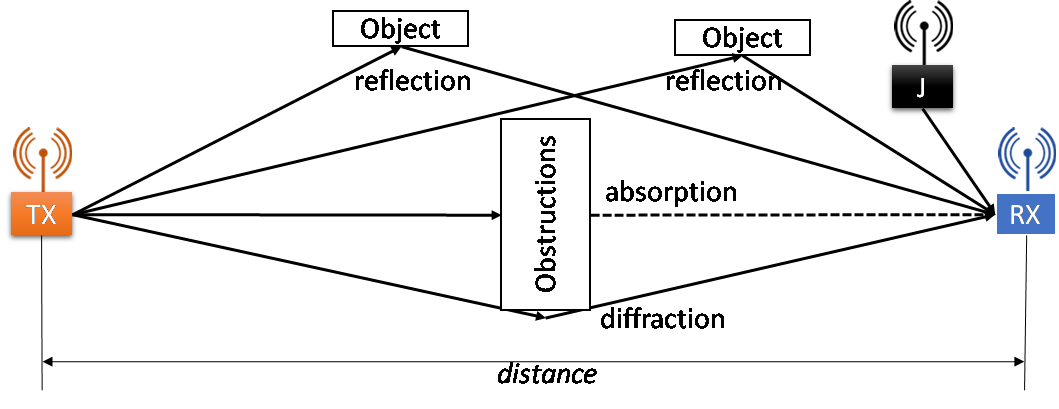
\includegraphics[width=0.6\textwidth]{chapter-intro/images/multipath}
	\caption{Wireless range, obstructions, absorption, reflection, diffraction, and jamming}
	\label{intro:fig:multipath}
\end{figure}

\paragraph{Interference} Electromagnetic interference (EMI) is always present to some degree in a wireless network.  EMI when in the radio frequency spectrum creates a disturbance that disrupts intended communications.  The disturbance can degrade performance by introducing RF energy into the circuits of wireless devices.  When the disturbance is strong enough to overcome the intended signal, communication loss will result.  Sources of EMI include both man-made and natural sources.  Natural radio sources typically will not interfere with network operation as the devices or deployment locations are designed to accommodate some natural interference.  Man-made interference can include other competing radio devices that operate in the same frequency band or nearby in frequency.  Noise from rotating electrical motors can also occur and typically affects radio bands below 400 MHz.  Common interference sources include personal devices such as cell-phones in which the Wi-Fi hotspot is enabled.  It can also include non-communication devices such as micro-wave ovens.  EMI can also emanate from intentional radio jammers designed to disrupt communications, and this can be classified as a security issue.

\section{Wireless Key Performance Indicators}

Given the challenges described in the previous section, assessing the performance of the wireless system becomes a matter of defining and then measuring key performance indicators (KPI) relevant to the success of a given wireless deployment.  A KPI can be considered a requirement of an industrial system if that KPI is used to specify a condition or capability needed by a stakeholder to solve a problem or achieve an objective within the factory enterprise.  Requirements considerations for designing or implementing a wireless communication system in a factory workcell include latency, reliability, scalability, range, payload size, update rate, operation and implementation cost, security, and system resiliency. These requirements are important aspects of a wireless network~\cite{CandellRW2017}. These requirements have particularly influential roles in implementing a wireless communications system in a factory environment and then assess the success of a wireless deployment.  The following paragraphs define the key performance indicators (which may be considered as requirements) for an industrial wireless system. 

\paragraph{Latency}
Latency is defined as the period of time between information transmission and reception between two actors.  Most non-industrial wireless systems are designed for higher data rates without regard for latency. However, for industrial applications, low latency is an important factor in control-based tasks as transmissions that occur outside of the latency threshold are considered failed transmissions. Industrial applications use smaller packet sizes with precise timings, signifying the criticality of latency.
\begin{definition}[Latency] \label{def:latency}
	The time between transmission of the first bit of information to the time in which that information is received by its intended recipient.
\end{definition}

\paragraph{Reliability}
Industrial functions such as safety transmissions or critical control processes are examples of functions that require an extremely high degree of reliability because a “missing” transmission could have serious consequences to safety, production, and/or equipment integrity. High-reliability in industrial communication is crucial for numerous mission-critical applications. 

\begin{definition}[Reliability] \label{def:reliability}
	The probability of loss of information due to any source of noise or exceeded latency.
\end{definition}

\paragraph{Scalability}
Scale, in an industrial wireless point-of-view, is the number of devices that can be deployed on the network while retaining reliability, speed, and data-rate at set requirements. Scalability is important for dynamic networks where devices come-in and go-out of use. One distinct advantage of wireless communications is the ease with which nodes can be added to the network without the need for laying wire or cable.
\begin{definition}[Scale] \label{def:scale}
	The number of participating devices within a network.
\end{definition}

\paragraph{Range}
Range is the maximum distance to which a wireless link can extend while maintaining all other requirements. In general, as the distance of the wireless link increases, the channel losses increase and the signal power between nodes decreases. Excess range affects the reliability and latency of transmission. Specifically, in an industrial environment, meeting a required range specification is more challenging than an outdoor scenario due to increased path loss.
\begin{definition}[Range] \label{def:range}
	Range is the maximum distance to which a wireless link can extend while maintaining all other requirements
\end{definition}

\paragraph{Payload Size}
Payload size is the size, in bytes, of the information portion of a transmission; however, the payload excludes header, framing, and error-correction information. Differentiating the payload size from the overall individual packet size allows the designer to ascertain the size of the information portion of the transmission. Many industrial applications, such as safety and control applications, the payload size is small.
\begin{definition}[Payload Size] \label{def:payloadsize}
	The informational length of information to be transmitted not including all overhead associated with the protocol used for transmission.
\end{definition}

\paragraph{Update Rate}
Certain manufacturing applications require higher update rates to achieve desired workcell performance. A wireless network must be capable of supporting required update rates needed by all the applications on that wireless network. For example, a force feedback control application that utilizes a wireless force-torque sensor may require 125 Hz sample rate. An example of such an application may be found in reference~\cite{Candell_ISIT_2019}. Update rate is an important factor that impacts the deployment and configuration of wireless networks and it dictates the effectiveness of frequency planning~\cite{Candell2018.IWSGuide}.
\begin{definition}[Update Rate] \label{def:updaterate}
	Rate of transmission for a particular process variable.
\end{definition}

\paragraph{Operation and Implementation Costs}
A consideration for implementing industrial wireless communications is the cost savings. For a wireless communications system, there is no need to install and, later, replace cabling due to degradation and wear. In wireless communications, redundancy can be achieved without cables. Wireless communications require lower labor costs as remote monitoring and control extend the ability to monitor and manage remote sites; onsite personnel is unnecessary. Electricity cost is lower for wireless installations, due to the relatively low power draw of wireless communications.

\paragraph{Security}
Security in wireless communications is not equivalent to security in wired communications in that wireless networks offer a different potential for exploitation; wireless uses air for communication which provides easier access to remote foreign actors. Along with the threat of remote jamming, there exists the possibility, absent adequate security protection, that wireless networks could be accessed if the keys to the public-key cryptography are discovered and encrypted transmissions are revealed. Wireless for industrial applications must be reliant to security related threats as the loss of communication can be costly and may damage equipment or personnel. Detailed requirements for wireless security are not discussed further in this report but more information can be found in~\cite{Stouffer2015}.

\paragraph{System Resiliency}
Overall system resiliency in a factory environment must be considered as issues with networking may lead to unnecessary inefficiency. For example, if power is disrupted a network must be able to reestablish connectivity within seconds. Intelligent applications may also be required to overcome network communication issues. Achieving a resilient network is not trivial as current wireless device may require long periods of time to reestablish connections within the network.  For example, mesh networks based on low-data-rate protocols can often take minutes to reestablish an operational network after an intermittent loss of power.  System resiliency is outside the scope of this report; however, system resiliency issues such as recovery time after power loss must be considered in the design of wireless technology for use in factory workcells.

\paragraph{Power and Battery Life}
Often overlooked is the power efficiency of wireless devices.  In factories in which power is readily available such as in a workcell or on a mobile cart platform, power efficiency is not often considered.  In scenarios where devices are deployed over large distances such as in a oil refinery or water purification plant, battery life becomes important.  Battery life can also be important for large scale deployments in factories with thousands of devices.  In those scenarios, the frequency of battery change or failure can drive costs substantially.  Therefore, power efficiency and the impact of design factors on battery life can be equally as important as reliability in a deployment. 


These requirements vary greatly depending on the class of industrial application and much work has been done to try to make sense of the classes of applications and there subsequent requirements.  An illustrative perspective of these is given in Fig.~\ref{intro:fig:wirelesspecs} showing both typical and worst case specifications.  


\begin{figure}[!tbp]
	
	\centering
	\begin{subfigure}{.8\textwidth}
		\centering
		% include first image
		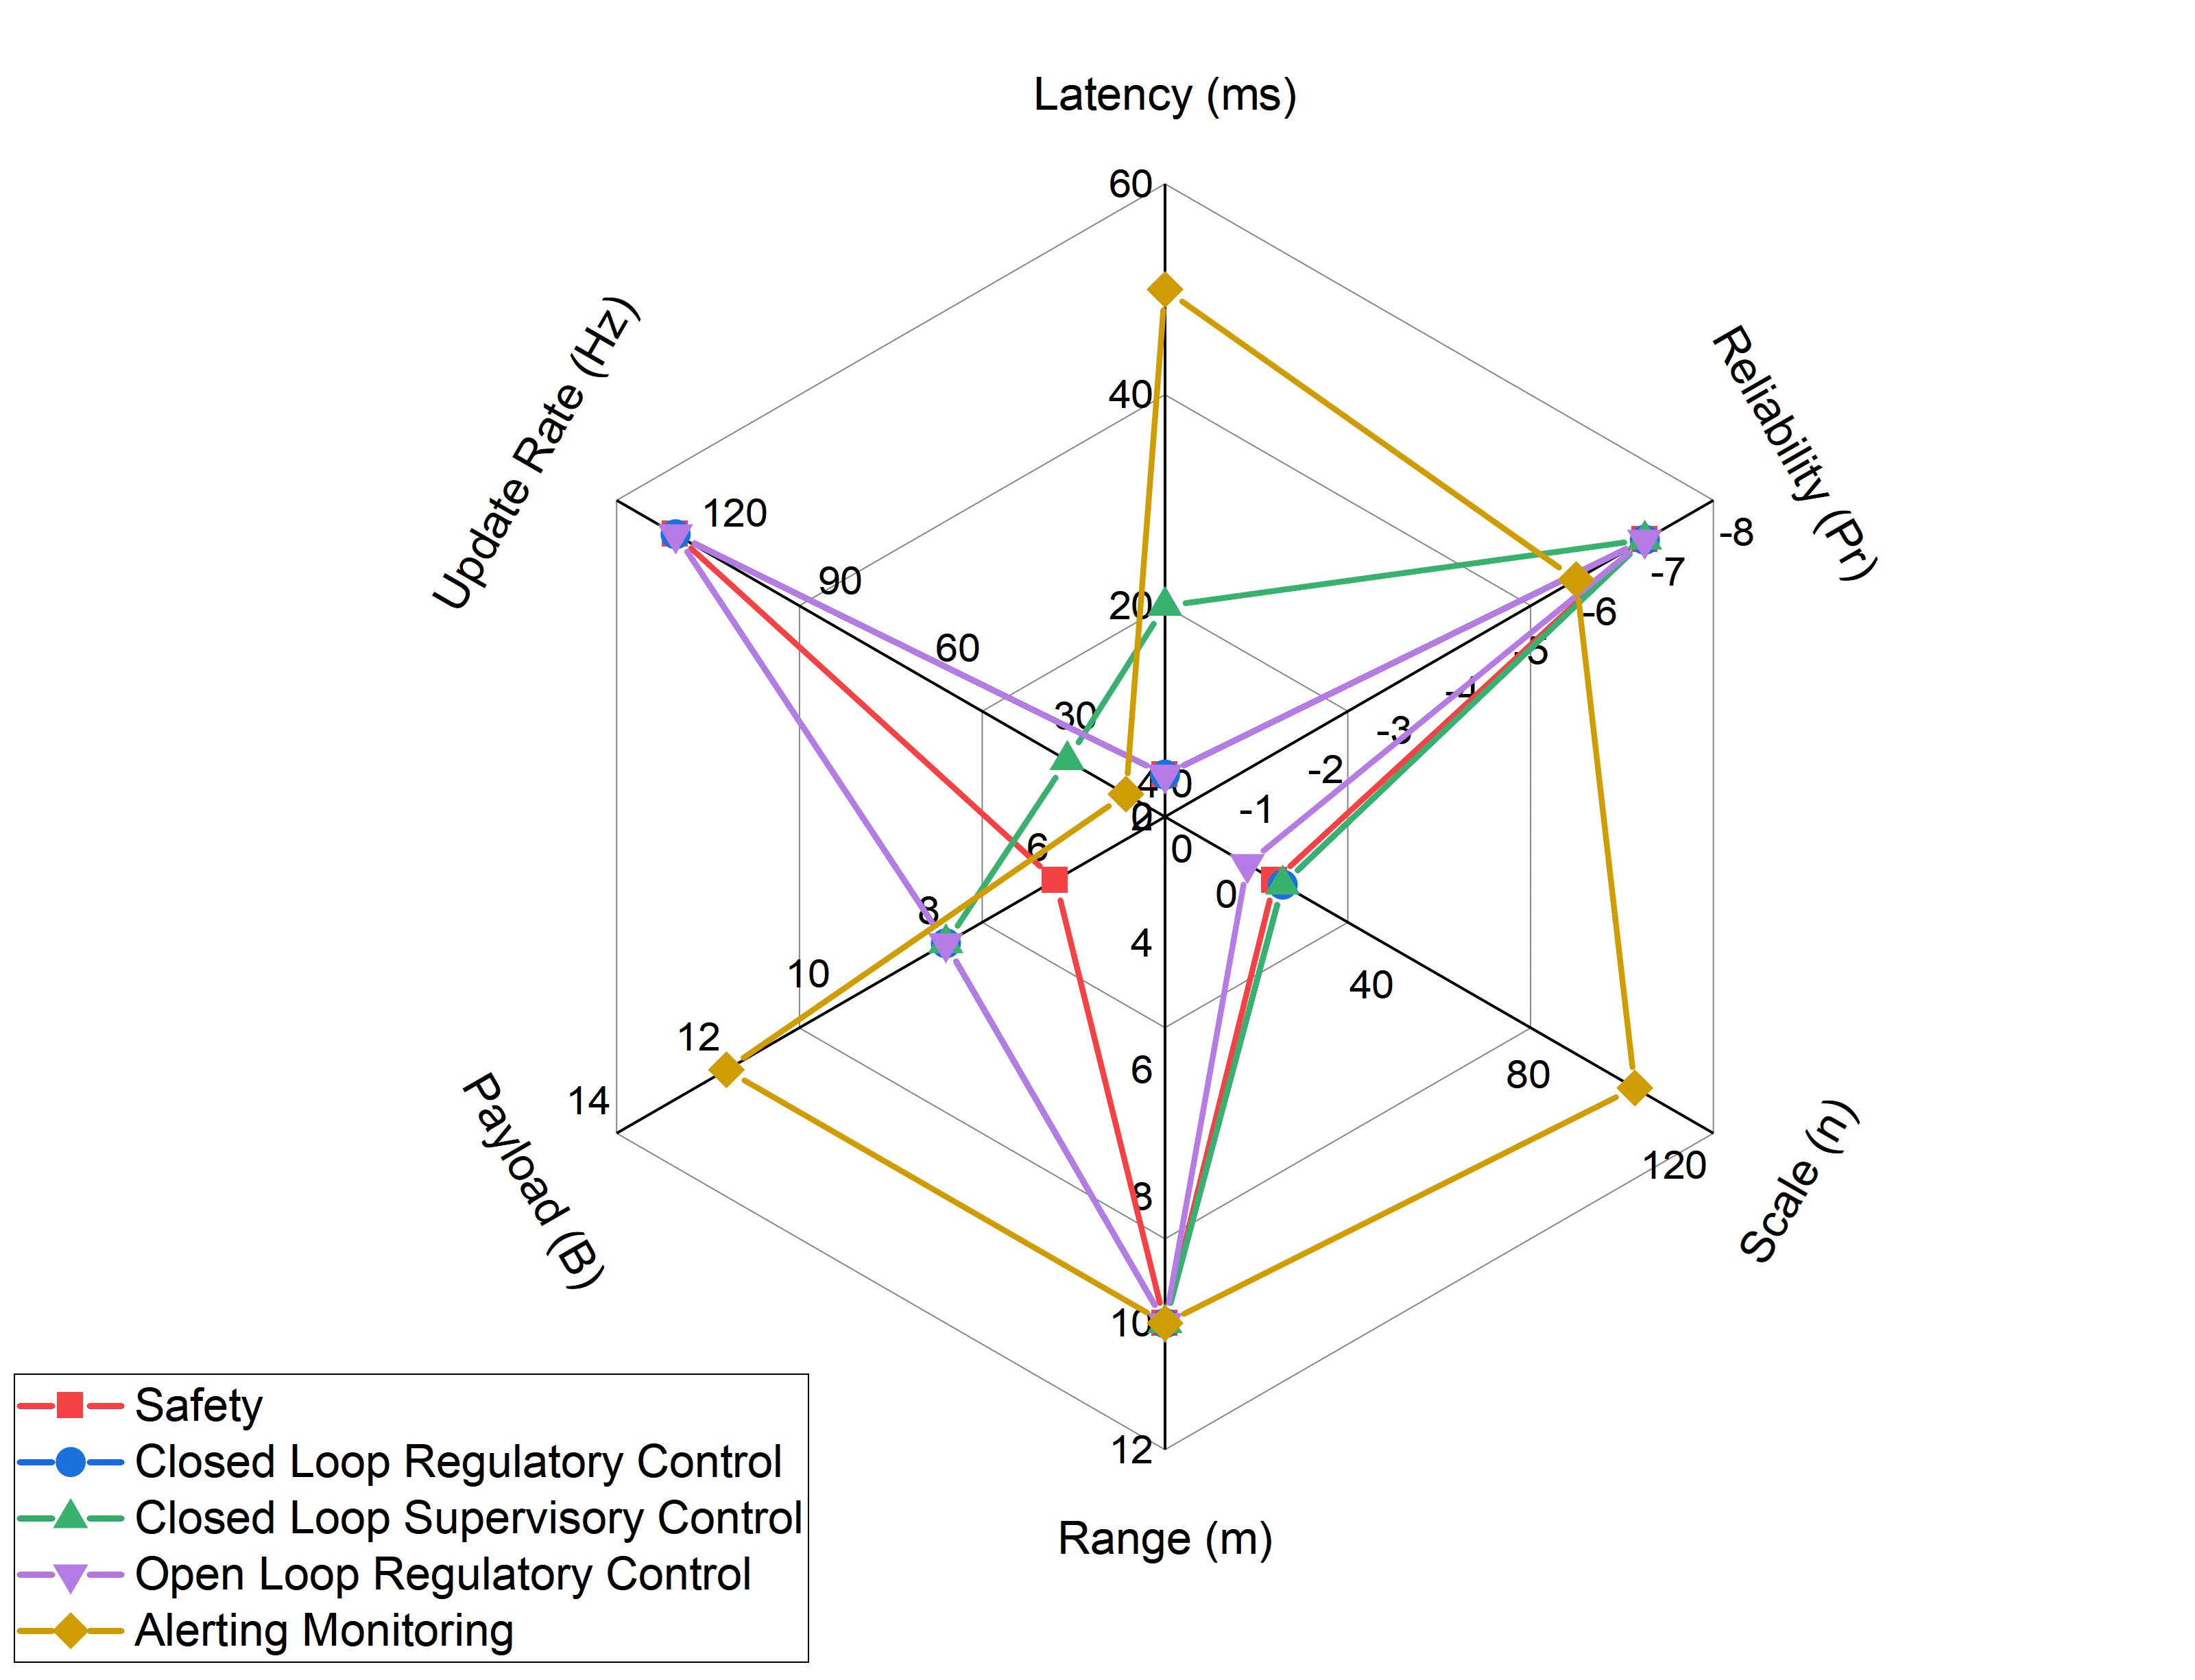
\includegraphics[width=.95\textwidth]{chapter-intro/diagrams/TypicalSpecs}  
		\caption{Typical}
		\label{intro:fig:typicalspecs}
	\end{subfigure}
	\begin{subfigure}{.8\textwidth}
		\centering
		% include second image
		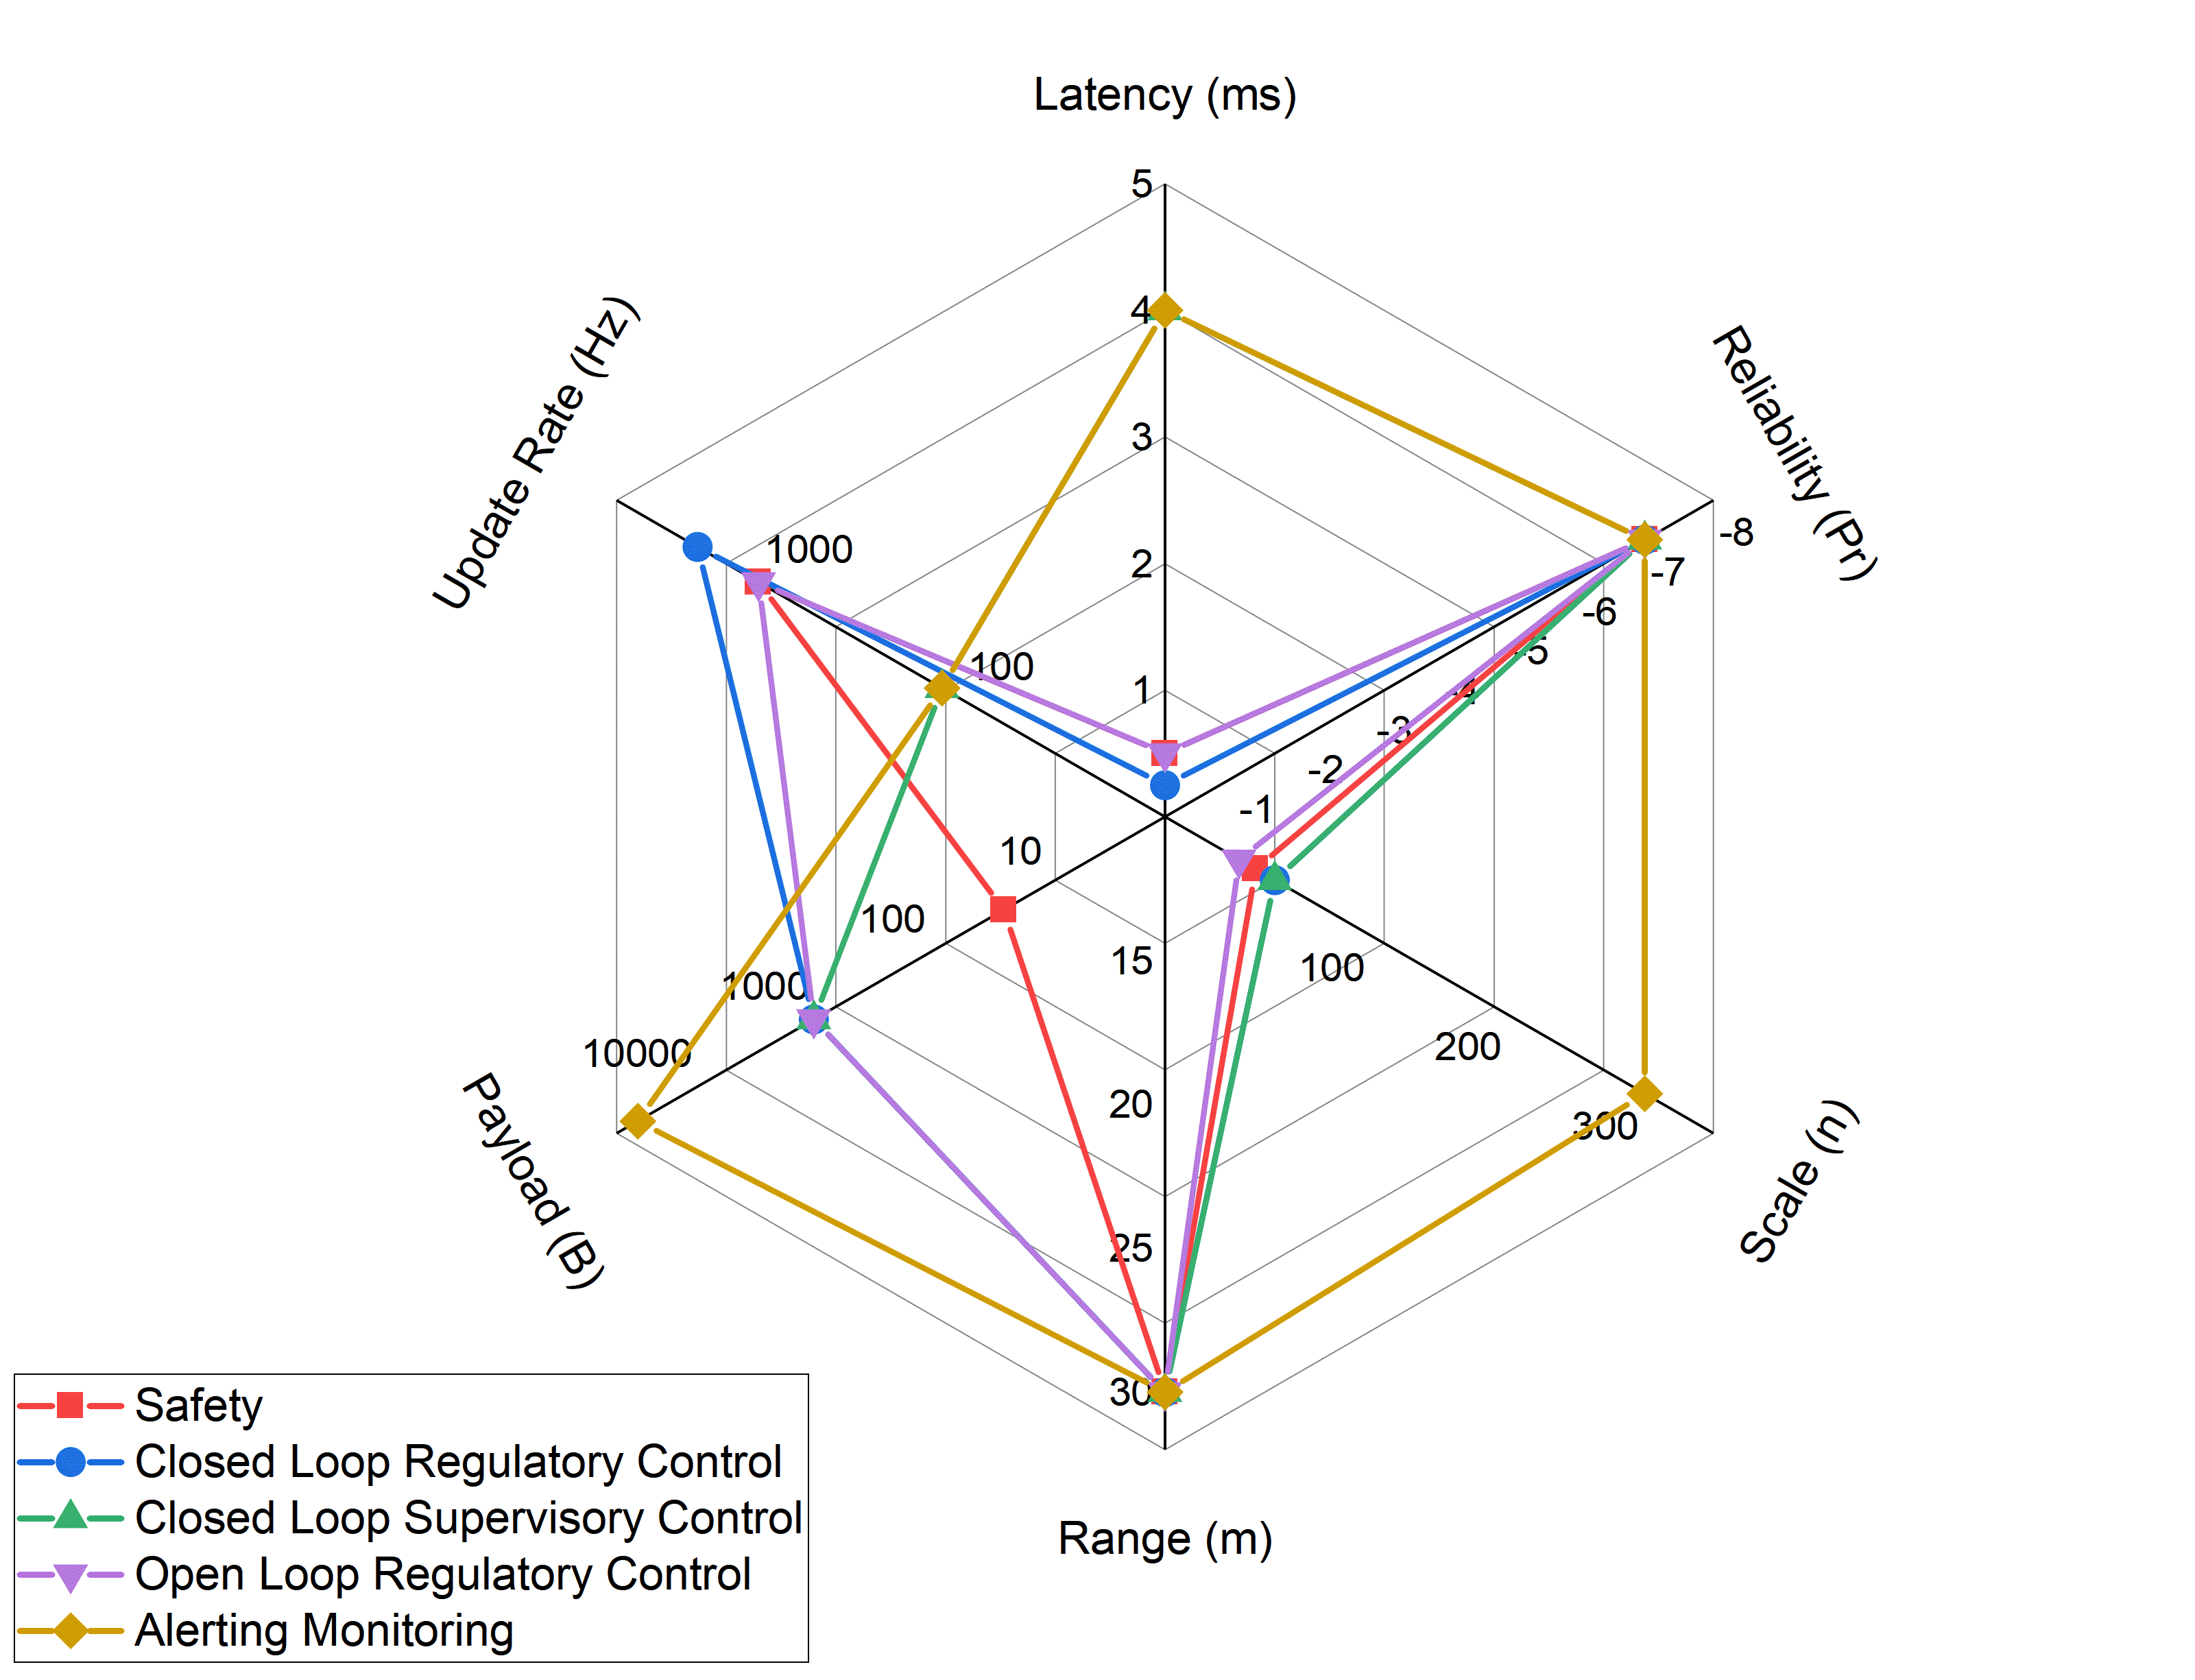
\includegraphics[width=.95\textwidth]{chapter-intro/diagrams/WorstSpecs}  
		\caption{Worst Case}
		\label{intro:fig:worstspecs}
	\end{subfigure}
	\caption{
		Typical ~\protect\subref{intro:fig:typicalspecs} and Worst Case ~\protect\subref{intro:fig:worstspecs} key performance indicators for industrial wireless use cases presented in~\cite{Montgomery2019}.
	}
	\label{intro:fig:wirelesspecs}	
	
\end{figure}



\section{Performance Evaluation}

The focus of the research presented in this body of work is the estimation of performance of cyberphysical systems....

Present the TESTBED!!!

A clearer concept of the requirements will not only allow for the development of realistic wireless systems, but it is also essential in the construction of more accurate models, the conduct of more effective testing, and better analysis the performance measurement data that results.

First understanding the technical landscape: components, interfaces, and constraints

Next setting up a framework for performance evaluation: use case definition, testbed abd data capture, organization of data captured, 

Analysis methods for the captured data: data cleaning, curation, and application of the graph database

Application of machine learning as an example and how different algorithms performance to inferring an important metric in industrial wireless, i.e., signal to interference level

Performance is often done as a before and after; however some effort has been made to standardize test methods~\cite{Candell2015, Candell2017IWW}

\section{Thesis Organization}

\blindtext



